\chapter{Indoor and In-field Measurements} 
\label{ch:measurements}

In this chapter, we introduce the in-field measurements in Dallas-Fort Worth 
Metroplex and mobility footprint of WiEye Global measurements. 
We analyze these measurements in channel utility and user mobility for 
further research.


%context information experiments
\section{In-lab Experiments for Radio Characterization}
\label{subsec:ichannel}
To establish an SNR-to-throughput relationship, we first use an experimental setup where two 
wireless nodes communicate across repeatable emulated channels generated 
by the channel emulator (Figure~\ref{fig:in-door experiment}). For a given band and card, we measure
the throughput of a fully-backlogged UDP flow using the {\it iperf} 
traffic generator. We use constant attenuation over an idealized
channel condition and repeat the experiment to
produce various RSSI values.
Despite the same physical and media access control layers of the radios, there are
slight differences in the throughput achieved per radio at the same attenuation
level.  Thus, we normalize these throughput values to have the same maximum
throughput across radio types.
%for a fair comparison of the frequency bands.

\begin{figure} [h]
%\vspace{-0.1in}
\centering
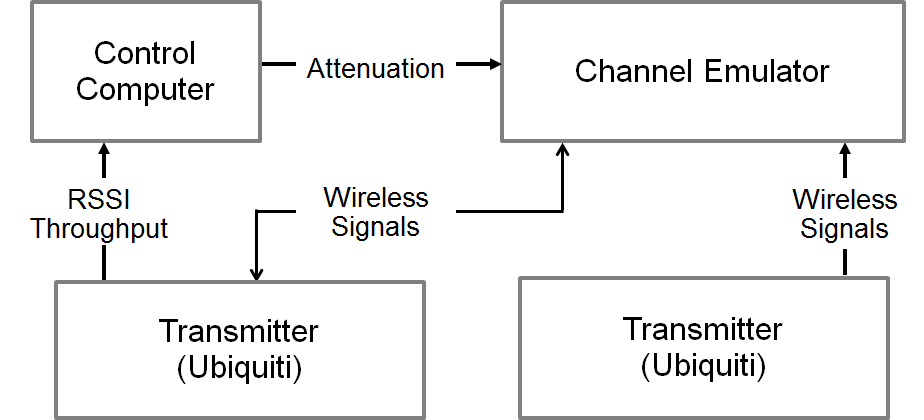
\includegraphics[width=85mm]{figures/emulator2}
%\vspace{-0.1in}
\caption{Experimental setup for channel emulator.}
\label{fig:in-door experiment}
\vspace{-0.1in}
\end{figure}





\section{In-field Measurements in DFW Metroplex}

We now describe the in-field experimental design to obtain a data set for
evaluating our multiband algorithms. 


\subsection{Iterative In-field Data Collection}
\label{subsec:insitu}

We perform measurements in a public park near SMU campus to collect repeated 
data set for evaluating our vehicular algorithms.
Two Gateworks boards, each containing
the aforementioned four radios, are installed on two cars.  One node is always
the receiver and at a fixed location. The other node is always the 
transmitter and travels 
around the block of a public park as shown in Figure~\ref{fig:infield}.
One loop of the route will be used as a unit of training in the next section.

\begin{figure} [h]
%\vspace{-0.1in}
\centering
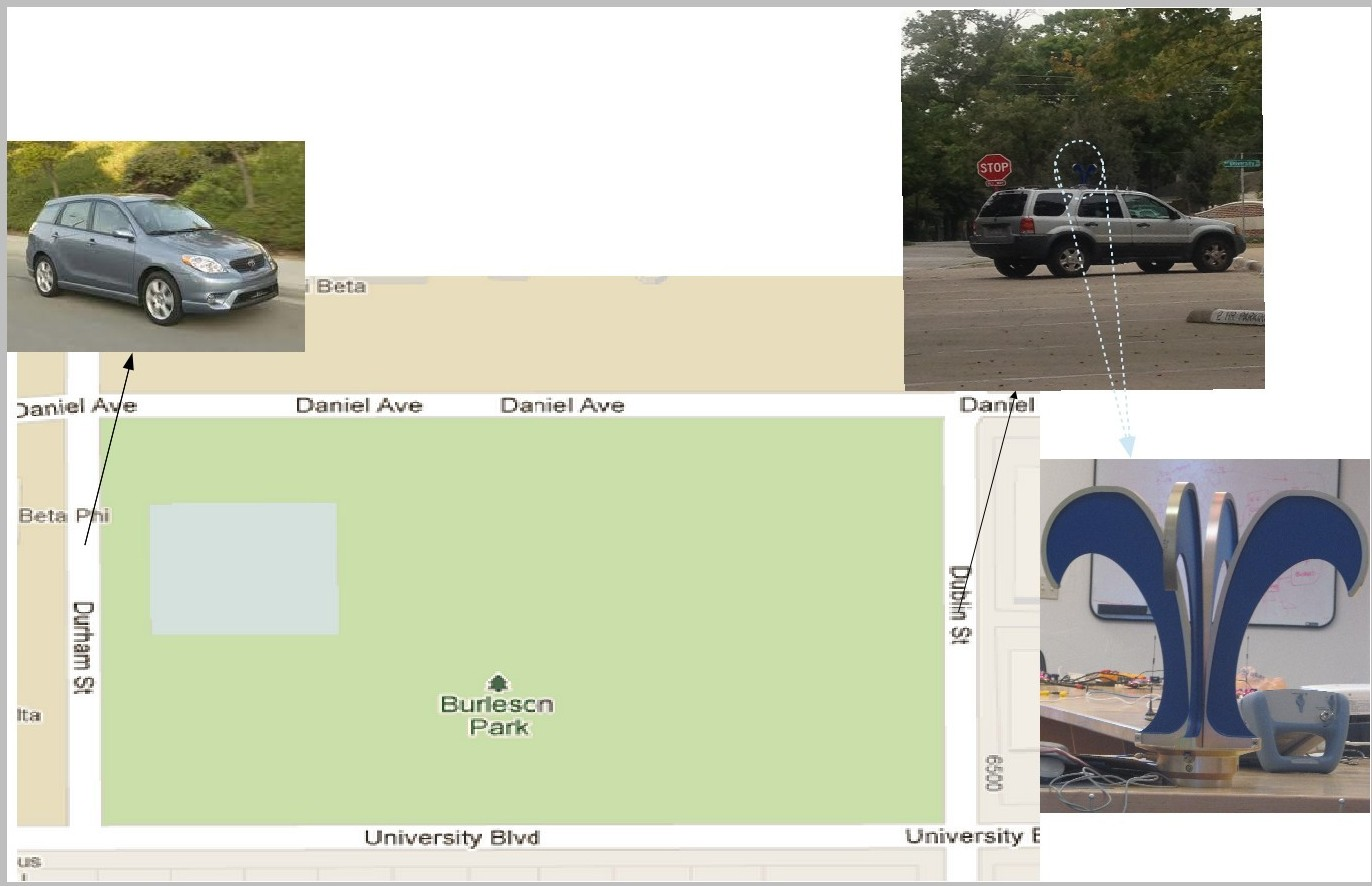
\includegraphics[width=85mm]{figures/infield}
\vspace{-0.1in}
\caption{In-field Experimental Setup.}
\label{fig:infield}
\vspace{-0.1in}
\end{figure}

During each loop, the transmitter sends a fully-backlogged UDP flow
using {\it iperf} on each of the four radios simultaneously.  To
focus on band selection and ensure the greatest range, we disable autorate and use a fixed data rate
of 6 Mbps. The receiver continually performs a {\it tcpdump} of all
received 802.11 packets~\cite{jacobson1989tcpdump}. Additionally, a
QH 400 Quad Ridge Horn Antenna (shown in Figure~\ref{fig:infield}) is 
connected to a Rhode \& Schwarz FSH8 mobile spectrum analyzer at the 
receiver to monitor spectral activity. Then, based on the 
time stamps, we remove 802.11 packets from the spectral trace 
so that only non-802.11 interference will contribute to $P_N^i$.

\begin{figure} 
%\vspace{-0.1in}
\centering
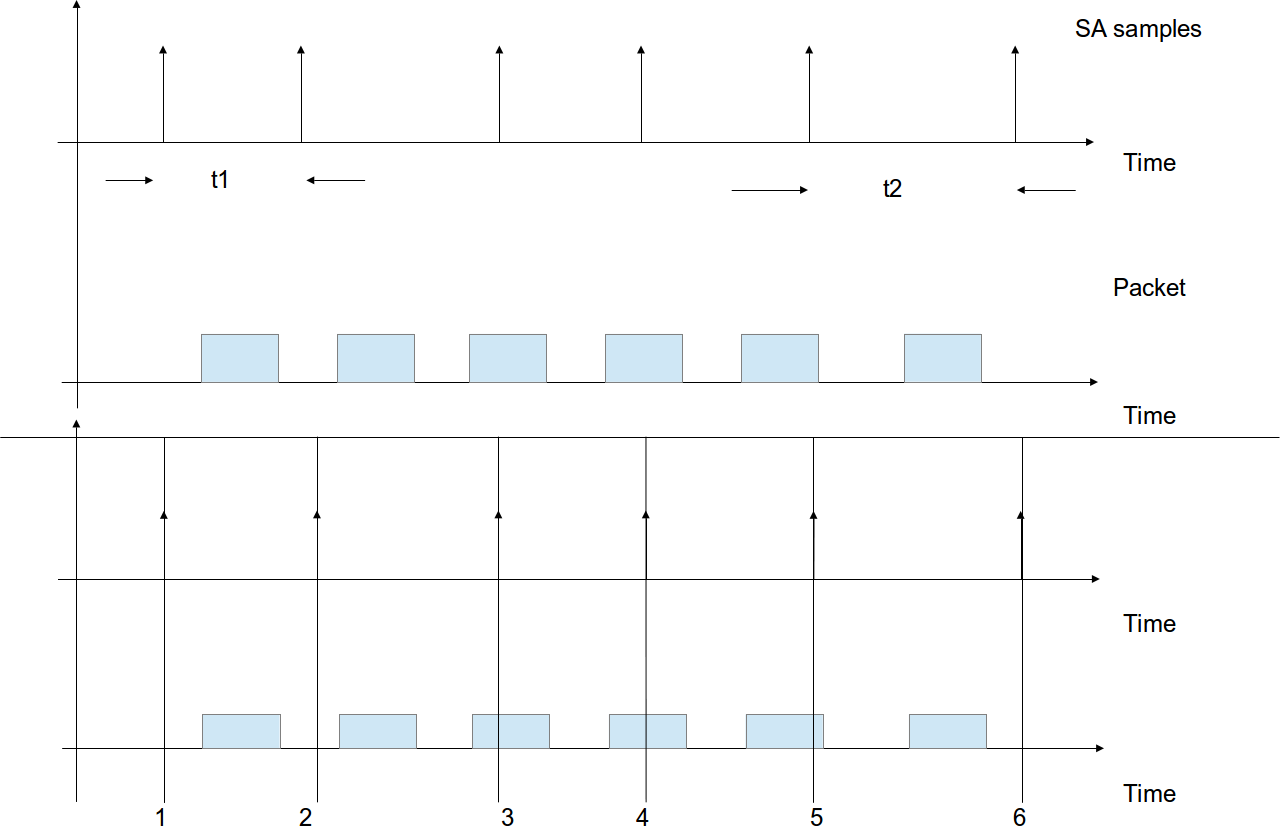
\includegraphics[width=85mm]{figures/sa_process}
\vspace{-0.1in}
\caption{Spectrum Analyzer Data Processing.}
\label{fig:sa_process}
\vspace{0.1in}
\end{figure}

Figure~\ref{fig:sa_process} shows how we obtain the
non-802.11 interference, $P_N^i$. We expunge the spectrum analyzer
(SA) samples which overlap in time with the dumped 802.11 packets,
such as packets 3, 4, and 5. Then, the reported interference value
will not contain the received power from 802.11 packets, which have
already been considered via the activity level, $A$.

The in-field data is processed offline where data from all instruments
involved is synchronized based on the GPS time stamps. 
As discussed in Section~\ref{subsec:ichannel}, the throughput of each radio
is normalized based upon emulator experiments to account for any
manufacturing differences.


% WINMEE

\subsection{Large Scale In-field Measurements in DFW Metroplex}
% Platform
%To ensure the results are applicable, 
%We employ a Linux-based 802.11 testbed, which includes a Gateworks 2358 board with 
%Ubiquiti XR radios (XR9 at 900 MHz, XR2 at 2.4 GHz, XR5 at 5.2 GHz) and a DoodleLabs DL475 
%radio at 450 MHz.  
%We develop shell scripts which utilize tcpdump to enable the testbed to
%work as a sniffer, recording all 802.11 packets. 
%However, since the Gateworks platform only 
%updates its estimate of received signal strength upon the reception of a new packet (and
%not all relevant channel activity is 802.11 based), we employ a spectrum analyzer to form 
%a notion of inter-network interference with finer granularity.  Hence, we also use a Rohde \& Schwarz FSH8 
%portable spectrum works from 100 KHz to 8 GHz. The portable spectrum analyzer is controlled 
%by a Python script on a laptop to measure the received signal strength.

We employ our Linux-based testbed, Rohde \& Schwarz FSH8 protable spectrum analyzer perform 
channel state measurements in multiple locations of DFW metroplex.
We develop shell scripts which utilize tcpdump to enable the testbed to
work as a sniffer, recording all 802.11 packets. 

%We perform experiments in downtown Dallas, SMU campus, and neighborhood. The results show
%no 802.11 packets detected in white space bands(450 MHz, 900 MHz) there. 
%And in DFW area, as far as we know, we are the only group holds FCC license of white space bands. 
%Our experiments verify that these bands have not been used for commercial wireless data communication.
%Moreover, we observed that Gateworks platform only update its received signal strength when received
%a new packet.
%It is not good for inter-network interference measurement. To cover the gap,
%we employ a spectrum analyzer, multiband antenna, mobile antenna and a laptop developing
%a spectrum sensing system.

% Data normalize 
To the best of our knowledge, there is no readily available mobile, multiband antenna from
450 MHz to 5.2 GHz on the market. Thus, we use a 700-MHz mobile antenna to perform in-field
measurements. We then normalize the mobile antenna performance across bands with indoor 
experimentation. To do so, we use a Universal Software Radio Peripheral (USRP) N210 to 
generate signals at 450 MHz, 800 MHz, and 2.4 GHz. We feed the USRP signals directly
to a spectrum analyzer and adjust the configuration of USRP to make the received signal 
strength the same as the 5.2 GHz signal from Gateworks 2358 with a XR5 radio. Then, we connect 
the signal source to a fixed multiband antenna (QT 400 Quad Ridge Horn Antenna) and measure the
received signal at a fixed distance with the 700 MHz antenna and antennas for different bands
to obtain the antenna loss for each band. We adjust the received signal strength
collected via the 700-MHz mobile antenna according to the normalization.

  \begin{figure}
  %\vspace{-0.0in}
  \centering
  \includegraphics[width=85mm]{figures/equipment}
  \vspace{-0.1in}
  \caption{Multiband Measurement Platform}
  \label{fig:equipment}
 % \vspace{0.1in}
  \end{figure}
  
% Duplicate measurement in WiFi
Our experimental platform is shown in Figure~\ref{fig:equipment}.
The mobile spectrum analyzer records 32 samples per second on each band under test with 
appropriate time stamps.
The Gateworks sniffer platform also records all the received WiFi packets according to their time stamps. 
The duplicate samples in WiFi bands from spectrum analyzer and Gateworks are deleted 
according overlapping time stamps. Accordingly, we calculate the activity level in WiFi bands. 
The activity level of white space bands is calculated solely based upon the spectrum analyzer measurements.  

% Location and Process 
%We apply drive test carrying our platform from Dallas to Weatherford as shown in~\ref{sec:problemformulation}.
%We choose experiments locations according to the population distribution in DFW metropolitan. 
%The experiments are performed in Dallas, Weatherford and Millsap marked with stars in 
%Figure~\ref{fig:drivemap}.
Figure~\ref{fig:drivemap} depicts a map of the available white space channels with
markers where we performed measurements in North Texas. To be representative of a broad range of
community types, we consider populations of approximately 25 times one another according to the
2010 U.S. Census, Millsap (500), Weatherford (25K), and Dallas (1.25 M).
We have collected measurements at multiple types of locations in Dallas, including a downtown area,
a residential area, and a university campus. In Weatherford and Millsap, we monitor wireless activities 
in three locations for 45 continuous minutes on a weekday in downtown, residential, and non-residential areas.
Then, we post-process the data to calculate the activity level of each band in each location.
First, we parse the SNR from the data logs via Perl scripts. Second, we merge the data from the two platforms
according to their respective time stamps and calculate the activity level of each band across these
locations. The activity level is then included in our framework as input parameter.

As an initial experiment, we perform a drive test from Dallas to Weatherford with cruise control 
set to 60 MPH while on the highway. The result of the in-field spectrum drive test is shown in 
Figure~\ref{fig:drivetest} according to the location and time of the measurement.
The measured activity via RSSI of 450 MHz is high in downtown Dallas and Fort Worth 
but has less signal activity in the urban and rural area between these city centers.
The low activity detected in the WiFi bands is due to the distance from the highway being typically
larger than the propagation range of predominantly indoor wireless routers.
%The map depicted in Figure~\ref{fig:drivemap} shows the available white space channels in DFW area, more green means
%more channels. 
Our initial in-field measurement matches the FCC restrictions (shown in Figure~\ref{fig:drivemap}) with
less channels available translating to greater spectrum utilization by TV stations.
The drive test also shows that the spectrum utilization is roughly proportional to the population
density in Figure~\ref{fig:drivetest}. We use the measurements collected at more fixed locations as marked on the map for
the activity level calculation. 

\begin{figure}
%\vspace{-0.0in}
\centering
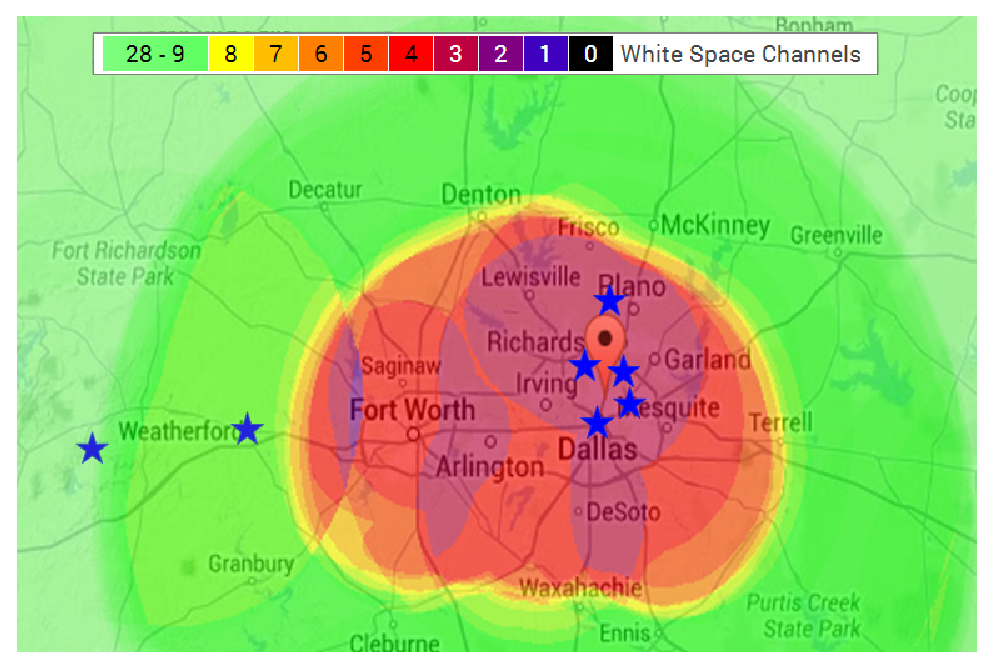
\includegraphics[width=85mm]{figures/drivemap}
%\vspace{-0.05in}
\caption{White Space Channels in DFW Metropolitan and Surrounding Areas.}                                                                 
\label{fig:drivemap}
\vspace{0.1in}
\end{figure}
   
\begin{figure}
%\vspace{-0.0in}
\centering
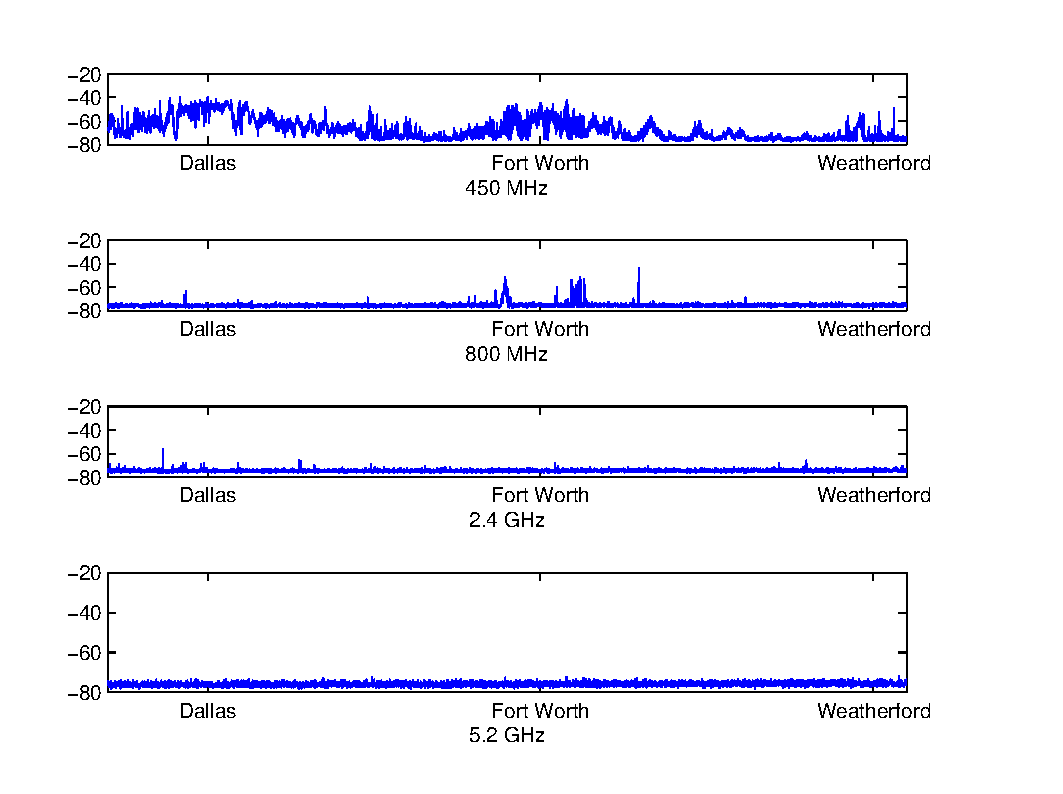
\includegraphics[width=94mm]{figures/drivetest}
%\vspace{-0.4in}
\caption{Spectrum Activity in DFW Metropolitan and Surrounding Areas.}                                                                 
\label{fig:drivetest}
%\vspace{0.1in}
\end{figure}

The activity level calculated with our measurements are shown in Table~\ref{tab:activitymeasurement}.
Dallas, the city with the greatest population in North Texas, has the highest activity level in most 
of the measured bands, especially at 450 MHz. The Dallas urban measurements are taken from the SMU 
campus, two neighborhoods, and a densely-populated suburb (Plano). Our measurements indicate that 2.4 GHz 
has a higher activity level in urban area than the measured downtown area. Most schools and their 
neighborhoods are covered by WiFi, which contributes to the high activity level at 2.4 GHz and 5.2 GHz.
In Weatherford, all the bands have lower activity levels than in Dallas. A peculiarity in the measurements
can be seen by the sparse area in Weatherford having more activity than the other regions for 450 MHz.  
This can be explained due to the measurement location being on the East of Weatherford (closer to Fort Worth,
which has a population of approximately 750k).
Millsap is a typical sparse rural area with approximately 500 total residents. The activity levels across 
all the bands are lower than in Dallas and Weatherford. In the 450 MHz band, the activity level decreases 
much faster than in other bands in Dallas and Weatherford. 

\begin{table*}
\centering % centering table 
\begin{tabular}{|l|c|c|c|c|c|c|c|c|} % creating 12 columns 
\hline %\hline % inserting double-line 
Bands     & \multicolumn{3}{c|}{Dallas} & \multicolumn{3}{c|}{Weatherford} \\% [0.5ex]
\hline % inserts single-line 
% Entering 1st row 
Area Type & Downtown & Residential & Suburban & Downtown &  Residential & Sparse \\ % [0.5ex]
\hline % inserts single-line 
450 MHz &24.37	&25.83  &23.77	&6.05 &12.50  &14.03  \\      
\hline % inserts single-line                                                                                                       
800 MHz &4.40 	&16.49  &4.77	&5.22&5.07 &4.43   \\      
\hline % inserts single-line                                                                                                      
2.4 GHz &15.87 	&34.95  &2.60	&2.03&2.03 &2.77   \\      
\hline % inserts single-line                                                                                                     
5.2 GHz &19.70	&35.46  &1.53	&1.93&1.93 &1.33   \\      
\hline % inserts single-line 
\end{tabular}    
\caption{Activity Level in Dallas \& Weatherford} % title name of the table 
\label{tab:activitymeasurement_d_w}    
\vspace{-0.1in}
\end{table*}    

\begin{table*}
\centering % centering table 
\begin{tabular}{|l|c|c|c|c|c|} % creating 12 columns 
\hline %\hline % inserting double-line 
Bands     & \multicolumn{3}{c|}{Millsap} \\% [0.5ex]
\hline % inserts single-line 
% Entering 1st row 
Area Type & Downtown & Residential & Sparse \\ % [0.5ex]
\hline % inserts single-line 
450 MHz & 7.00 & 0.07 & 0.02 \\      
\hline % inserts single-line                                                                                                       
800 MHz & 3.87 & 4.20 & 3.60 \\      
\hline % inserts single-line                                                                                                      
2.4 GHz & 2.07 & 1.60 & 0.80 \\      
\hline % inserts single-line                                                                                                     
5.2 GHz & 1.27 & 2.07 & 2.10 \\      
\hline % inserts single-line 
\end{tabular}    
\caption{Activity Level in Millsap} % title name of the table 
\label{tab:activitymeasurement_m}    
%\vspace{-0.3in}
\end{table*}    




% Whitecell
\subsection{Long Term In-field Measurements in DFW Metroplex}
\label{subsec:measurements}

We perform in-field measurements in typical areas to find the channel state variation across 
time and the user mobility patterns among the areas.
% 24 hours measurement introduction
We chose neighborhoods, campus, downtown business office and 
urban business office to perform long term 24 hours measurements on weekdays. 
The locations we chosen are located in Downtown Dallas, a university campus in Dallas, 
a business in Dallas urban area and an apartment on north Dallas. 
The locations where we collected measurements are shown in Fig.~\ref{fig:measurement_map}.

\begin{figure}
\vspace{-0.0in}
\centering
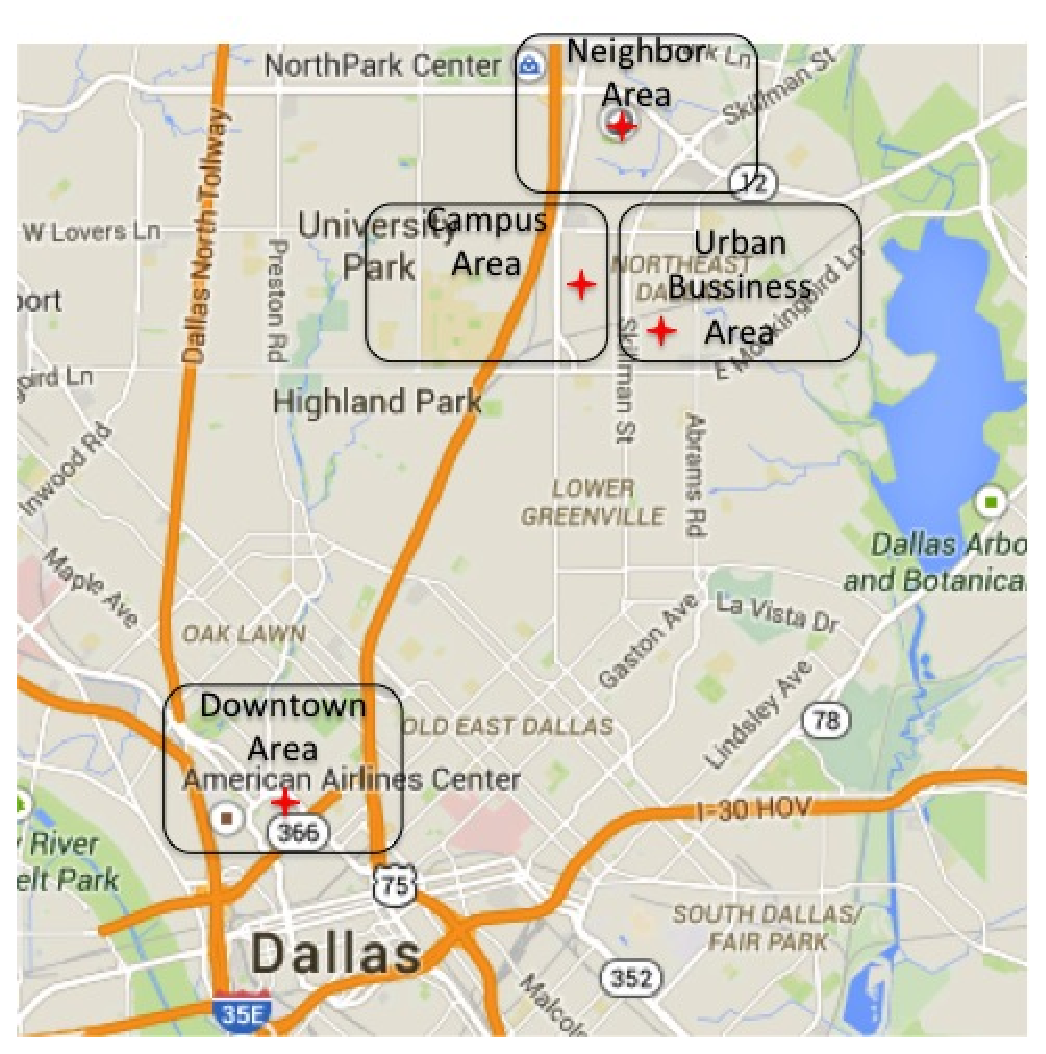
\includegraphics[width=84mm]{figures/measurements_map}
\vspace{-0.1in}
\caption{Long Term Measurements Locations}
\label{fig:measurement_map}
\vspace{-0.1in}
\end{figure}

In each of the location, we left our equipment running to measure the channel state for 24 hours during 
weekdays. 
% Experiment equipment
We employ a Rohde \& Schwarz FSH8 portable spectrum works from 100 KHz to 8 GHz. 
The portable spectrum analyzer is controlled by a Python script on a laptop to measure 
the received signal strength.
% Data normalize 
To the best of our knowledge, there is no readily available mobile, multiband antenna from
450 MHz to 5.2 GHz on the market. Thus, we use a 700-MHz mobile antenna to perform in-field
measurements. We then normalize the mobile antenna performance across bands with indoor 
experimentation. To do so, we use a Universal Software Radio Peripheral (USRP) N210 to 
generate signals at 450 MHz, 800 MHz, and 2.4 GHz. We feed the USRP signals directly
to a spectrum analyzer and adjust the configuration of USRP to make the received signal 
strength the same as the 5.2 GHz signal from Gateworks 2358 with a XR5 radio. Then, we connect 
the signal source to a fixed multiband antenna (QT 400 Quad Ridge Horn Antenna) and measure the
received signal at a fixed distance with the 700 MHz antenna and antennas for different bands
to obtain the antenna loss for each band. We adjust the received signal strength
collected via the 700-MHz mobile antenna according to the normalization.
We use $-85 dBm$ as a threshold in the activity level calculation for the normalized data.

% Introduce how to calculate the capacity
% Explain multiband and activity level
When wireless devices operate in WiFi bands, the channel separation is relatively 
small (e.g., 5 MHz for the 2.4 GHz band). As a result, many works assume that
the propagation characteristics across channels are similar. However, with the
large frequency differences between WiFi and white space bands (e.g., multiple GHz),
propagation becomes a key factor in the deployment of wireless networks with both bands.
Here, a frequency band is defined as a group of channels which have
little frequency separation, meaning they have similar propagation characteristics.
In this work, we consider the diverse propagation and activity characteristics
for four total frequency bands: 450 MHz, 800 MHz, 2.4 GHz, and 5.2 GHz.
We refer to the two former frequency bands as white space bands and
the two latter frequency bands as WiFi bands.
The differences in propagation and spectrum utilization create opportunities
for the joint use of white space and WiFi bands in wireless access networks according
to the environmental characteristics (e.g., urban or rural and downtown or residential)
of the deployment location.


Through the measured data set, we calculate the activity level via Eq.~\ref{eq:actdef}.
The activity level is calculated in one minute time window.
We average the activity level in 30 minutes across 24 hours.
% Need to discuss the \mu mapping with these measurements stuff



% FIXME how to show the data
\begin{table*}
\centering % centering table 
\begin{tabular}{|l|c|c|c|c|c|c|c|c|c|c|c|c|c|c|} % creating 13 columns 
\hline % inserts single-line 
\multirow{8}{*}{Downtown}	
&\multirow{2}{*}{450 MHz}	
&0:00-11:00 &  22.09 &  21.27 &  22.28 &  22.47 &  21.65 &  21.68&  22.37 &  22.16&  23.12 &  22.73&  22.01 &  22.54 \\ 	
\cline{3-15}	
&&12:00-23:00&  21.80 &  20.86 &  21.80 &  22.54 &  22.35 &  22.61&  22.45 &  21.58&  22.18 &  23.09&  22.11 &  22.09 \\ 	
\cline{2-15}	
&\multirow{2}{*}{800 MHz}	
&0:00-11:00 &  12.99 &  12.44 &  12.08 &  12.32 &  11.60 &  11.60&  12.48 &  12.10&  11.14 &  11.55&  11.98 &  11.12 \\ 	
\cline{3-15}	
&&12:00-23:00&  11.88 &  12.27 &  12.36 &  12.05 &  12.15 &  14.00&  13.32 &  12.29&  11.38 &  11.55&  12.92 &  13.16 \\ 	
\cline{2-15}	
&\multirow{2}{*}{2.4 GHz}	
&0:00-11:00 &  29.08 &  29.15 &  29.49 &  28.93 &  29.01 &  28.86&  28.84 &  29.53&  29.03 &  28.74&  29.89 &  29.15 \\ 	
\cline{3-15}	
&&12:00-23:00&  28.60 &  29.61 &  29.44 &  28.55 &  28.05 &  28.62&  28.74 &  28.93&  28.26 &  27.73&  28.19 &  29.85 \\ 	
\cline{2-15}	
&\multirow{2}{*}{5.2 GHz}	
&0:00-11:00 &  27.21 &  27.11 &  26.20 &  25.77 &  26.70 &  26.17&  25.67 &  26.10&  25.77 &  25.41&  26.05 &  26.34 \\ 	
\cline{3-15}	
&&12:00-23:00&  26.17 &  26.03 &  25.19 &  26.41 &  26.80 &  25.17&  26.08 &  25.60&  26.44 &  26.58&  25.50 &  25.45 \\ 	
\hline	
\multirow{8}{*}{Urban}	
&\multirow{2}{*}{450 MHz}	
&0:00-11:00 &  23.17 &  23.69 &  23.45 &  22.83 &  23.24 &  23.43&  23.48 &  23.74&  23.69 &  23.36&  23.29 &  23.00 \\ 	
\cline{3-15}	
&&12:00-23:00&  22.85 &  22.81 &  23.62 &  23.74 &  23.14 &  23.48&  23.38 &  22.52&  22.04 &  22.59&  22.59 &  22.42 \\ 	
\cline{2-15}	
&\multirow{2}{*}{800 MHz}	
&0:00-11:00 &  12.63 &  13.20 &  13.08 &  12.94 &  11.55 &  11.48&  11.60 &  11.38&  11.86 &  11.72&  10.47 &  10.32 \\ 	
\cline{3-15}	
&&12:00-23:00&  12.00 &  11.86 &  10.71 &  11.93 &  12.72 &  12.36&  11.48 &  11.43&  11.72 &  11.60&  11.72 &  11.91 \\ 	
\cline{2-15}	
&\multirow{2}{*}{2.4 GHz}	
&0:00-11:00 &  29.04 &  28.66 &  27.29 &  28.15 &  27.89 &  27.72&  28.18 &  27.38&  28.18 &  27.74&  28.15 &  27.96 \\ 	
\cline{3-15}	
&&12:00-23:00&  27.96 &  29.14 &  28.97 &  28.20 &  28.80 &  29.57&  29.02 &  27.72&  27.70 &  27.77&  29.21 &  28.42 \\ 	
\cline{2-15}	
&\multirow{2}{*}{5.2 GHz}	
&0:00-11:00 &  25.41 &  25.29 &  26.32 &  26.49 &  27.23 &  27.28&  26.99 &  26.27&  25.36 &  26.13&  25.81 &  24.88 \\ 	
\cline{3-15}	
&&12:00-23:00&  26.92 &  26.49 &  26.41 &  27.11 &  25.67 &  26.53&  26.73 &  26.97&  26.32 &  25.79&  27.57 &  26.65 \\ 	
\hline	
\multirow{8}{*}{Campus}	
&\multirow{2}{*}{450 MHz}	
&0:00-11:00 &  20.29 &  21.56 &  21.41 &  22.52 &  23.12 &  21.97&  21.65 &  21.63&  21.87 &  21.22&  21.17 &  21.39 \\ 	
\cline{3-15}	
&&12:00-23:00&  22.33 &  22.88 &  22.28 &  21.65 &  22.49 &  22.16&  21.32 &  22.35&  21.56 &  21.75&  21.75 &  20.45 \\ 	
\cline{2-15}	
&\multirow{2}{*}{800 MHz}	
&0:00-11:00 &  11.98 &  12.20 &  12.68 &  12.03 &  11.52 &  11.19&  11.96 &  12.94&  11.52 &  11.93&  12.44 &  10.95 \\ 	
\cline{3-15}	
&&12:00-23:00&  11.26 &  11.62 &  12.12 &  12.70 &  12.34 &  11.62&  11.57 &  12.17&  11.55 &  12.08&  11.88 &  11.98 \\ 	
\cline{2-15}	
&\multirow{2}{*}{2.4 GHz}	
&0:00-11:00 &  26.10 &  25.91 &  28.02 &  26.61 &  27.90 &  27.09&  27.01 &  27.21&  26.99 &  26.75&  25.69 &  26.46 \\ 	
\cline{3-15}	
&&12:00-23:00&  26.58 &  27.23 &  26.92 &  26.29 &  26.10 &  26.13&  26.25 &  25.53&  25.79 &  25.84&  26.13 &  26.46 \\ 	
\cline{2-15}	
&\multirow{2}{*}{5.2 GHz}	
&0:00-11:00 &  26.68 &  26.05 &  25.12 &  25.93 &  25.36 &  25.79&  26.03 &  26.73&  25.89 &  25.26&  25.81 &  25.50 \\ 	
\cline{3-15}	
&&12:00-23:00&  25.19 &  25.60 &  24.52 &  25.00 &  26.08 &  26.17&  26.85 &  26.53&  26.10 &  25.53&  25.89 &  25.31 \\ 	
\hline	
\multirow{8}{*}{Neighborhoods}	
&\multirow{2}{*}{450 MHz}	
&0:00-11:00 &  23.17 &  24.35 &  23.82 &  23.75 &  23.44 &  22.76&  24.08 &  25.26&  24.54 &  23.87&  23.82 &  23.70 \\ 	
\cline{3-15}	
&&12:00-23:00&  23.48 &  22.67 &  23.53 &  23.48 &  23.99 &  24.49&  23.99 &  22.98&  22.86 &  23.03&  23.89 &  23.63 \\ 	
\cline{2-15}	
&\multirow{2}{*}{800 MHz}	
&0:00-11:00 &  15.72 &  16.30 &  16.33 &  15.72 &  16.54 &  14.48&  14.62 &  14.48&  15.68 &  15.03&  15.60 &  16.33 \\ 	
\cline{3-15}	
&&12:00-23:00&  15.72 &  14.74 &  14.74 &  14.38 &  15.41 &  15.00&  15.84 &  16.25&  14.84 &  14.69&  15.51 &  14.93 \\ 	
\cline{2-15}	
&\multirow{2}{*}{2.4 GHz}	
&0:00-11:00 &  26.49 &  26.37 &  26.22 &  26.03 &  24.97 &  27.16&  27.76 &  26.56&  26.05 &  26.22&  25.74 &  27.18 \\ 	
\cline{3-15}	
&&12:00-23:00&  27.01 &  26.34 &  25.79 &  25.48 &  26.53 &  26.29&  25.33 &  25.86&  26.92 &  25.98&  25.48 &  27.66 \\ 	
\cline{2-15}	
&\multirow{2}{*}{5.2 GHz}	
&0:00-11:00 &  25.93 &  26.27 &  25.07 &  25.67 &  26.77 &  26.80&  27.52 &  25.38&  25.55 &  25.86&  25.62 &  26.13 \\ 	
\cline{3-15}	
&&12:00-23:00&  25.29 &  26.49 &  26.70 &  26.77 &  25.31 &  24.59&  24.78 &  25.91&  25.67 &  24.73&  24.73 &  25.21 \\ 	
%
%%Subtable here 
%\multirow{2}{*}{Downtown 450 MHz}	
%&0:00-11:00 &  22.09 &  21.27 &  22.28 &  22.47 &  21.65 &  21.68&  22.37 &  22.16&  23.12 &  22.73&  22.01 &  22.54 \\ 	
%\cline{2-14}	
%&12:00-23:00&  21.80 &  20.86 &  21.80 &  22.54 &  22.35 &  22.61&  22.45 &  21.58&  22.18 &  23.09&  22.11 &  22.09 \\ 	
%\cline{1-14}	
%\multirow{2}{*}{Campus 450 MHz}	
%&0:00-11:00 &  20.29 &  21.56 &  21.41 &  22.52 &  23.12 &  21.97&  21.65 &  21.63&  21.87 &  21.22&  21.17 &  21.39 \\ 	
%\cline{2-14}	
%&12:00-23:00&  22.33 &  22.88 &  22.28 &  21.65 &  22.49 &  22.16&  21.32 &  22.35&  21.56 &  21.75&  21.75 &  20.45 \\ 	
%\cline{1-14}	
%\multirow{2}{*}{Neighborhoods 800 MHz}	
%&0:00-11:00 &  15.72 &  16.30 &  16.33 &  15.72 &  16.54 &  14.48&  14.62 &  14.48&  15.68 &  15.03&  15.60 &  16.33 \\ 	
%\cline{2-14}	
%&12:00-23:00&  15.72 &  14.74 &  14.74 &  14.38 &  15.41 &  15.00&  15.84 &  16.25&  14.84 &  14.69&  15.51 &  14.93 \\ 	
\hline	
\end{tabular}    
\caption{Part of Activity Level in Multiple Locations} % title name of the table 
\label{tab:activitymeasurement}    
\vspace{-0.3in}
\end{table*}    


% Data analysis
% List part of the data
Through the activity level results, we observe that the activities of 450 MHz in the air has almost the same patterns across all 
the four measured areas. The large propagation area of 450 MHz influence the areas simultaneous and the 450 MHz activities are 
perform regularly on weekdays.
Neighborhood area has more activity in 800 MHz than other types of areas. But the 800 MHz activity levels are relatively lower than 
other bands in all the areas.
The WiFi 2.4 GHz channel of neighborhoods has more activity in the night while the downtown area has more activity in the day time.
The campus has more WiFi activities in the morning than the afternoon and night. 
Part of the measurements results are list in Table~\ref{tab:activitymeasurement}.
Due to the limited space, the full list of measurements are available upon request.
We integrate the measurements result into our numerical simulation of GSR algorithm later in this section.






\section{Mobility Footprint of WiEye Measurements}

% Here, discuss the wieye data process, 
We choose the data from WiEye database according to the GPS location. The data we chosen from
Dallas area, including downtown, urban, SMU campus and neighborhood area. We note the SMU campus 
area size as the unit, find the same size of downtown area and urban area. The rest of the chosen 
locations are counted as neighborhoods. The size of neighborhoods area is about $2.8$ of campus 
area. The data set is generated from Oct. 1st 2014 to March 20th 2015. 
We track the identified 538 users from the data set in different types of areas. 
The number of users located in these area are counted according to the GPS and further converted into 
the percentage each hour. The percentage distribution of users across these areas during a weekday is shown 
in Fig.~\ref{fig:wieyeprocess}

\begin{figure}
\vspace{-0.0in}
\centering
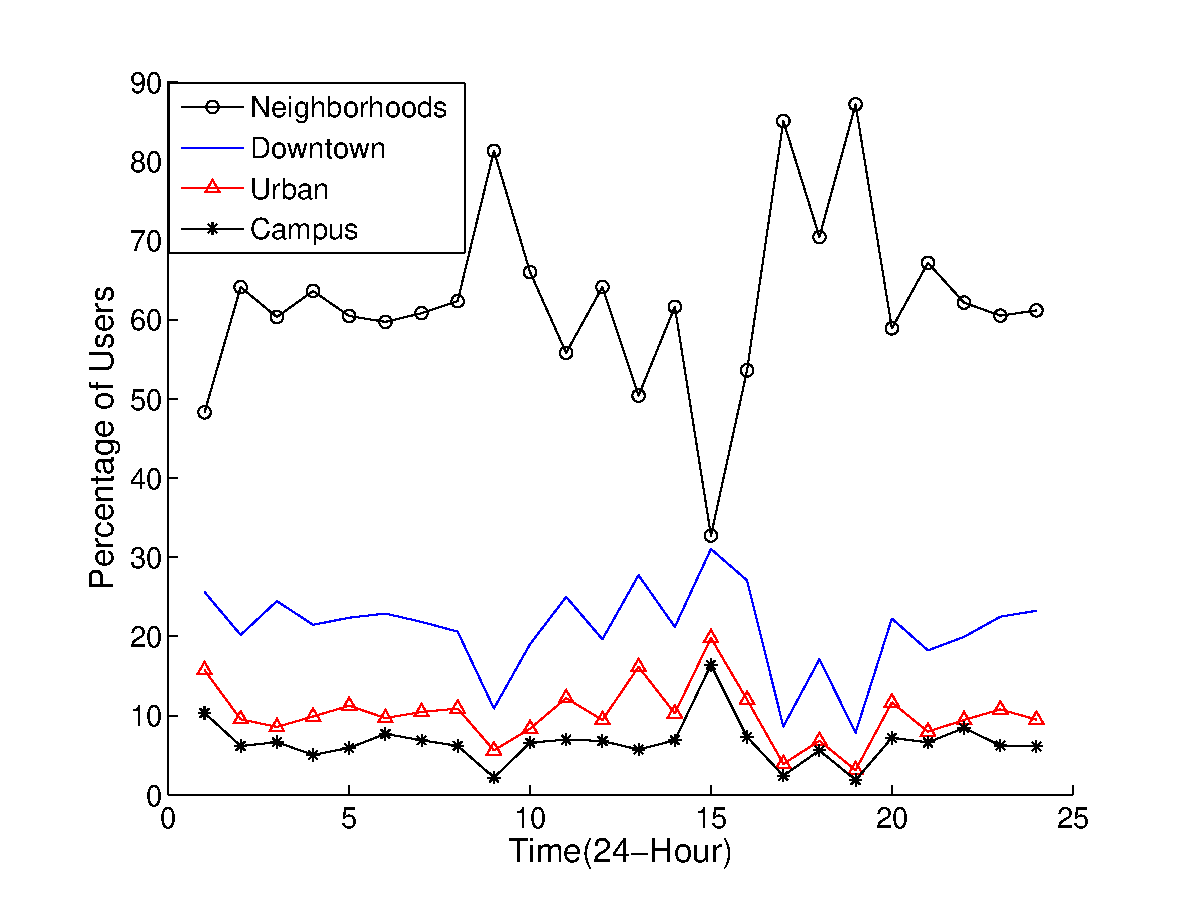
\includegraphics[width=84mm]{figures/wieyeprocess}
\vspace{-0.1in}
\caption{User Distribution across Time}
\label{fig:wieyeprocess}
\vspace{-0.1in}
\end{figure}

From the measurements results, we could find the distribution increase from 9:00 AM in the morning till 
3:00 PM in the afternoon in downtown, urban business area and campus. 
This match the most of the work schedule.
The peak of neighborhoods is around 6:00 PM in the afternoon and 9:00 AM in the morning. 
The reason could be the users are looking for breakfast in the morning before go to work.
We input the user mobility pattern into our power consumption numerical simulation.



